% **************************************************************************************************
% ** SPSC Report and Thesis Template
% **************************************************************************************************
%
% ***** Authors *****
% Daniel Arnitz, Paul Meissner, Stefan Petrik
% Signal Processing and Speech Communication Laboratory (SPSC)
% Graz University of Technology (TU Graz), Austria
%
% ***** Changelog *****
% 0.1   2010-01-25   extracted from report template by Daniel Arnitz (not ready yet)
% 0.2   2010-02-08   added thesis titlepage and modified layout (not ready yet)
% 0.3   2010-02-18   added TUG logo and statutory declaration
% 0.4   2010-02-18   moved the information fields below \input{./base/packages} (encoding...)
% 0.5   2010-03-02   added \ShortTitle to fix problems with long thesis titles
%                    added \ThesisType (makes the template suitable for MSc, BSc, PhD, ... Thesis)
% 0.6   2010-06-05   added pagestyle and pagenumbering after frontmatter, packages has now type
% 0.7   2010-09      \Advisors -> \Assessors, inserted frontmatter for thesis
% 0.8   2010-11      added examples
% 0.9   2011-04      \Twosided now {true,false}, scrbook for thesis (\front-, \main-, \backmatter)
%                    added \SpecialNote for titlepage (funding, etc.), added type "homework"
% 0.10  2011-10-18   fixed two typos in \bibliographystyle{} (bug reported by Michael Tauch)
% 0.11  2011-11-09   fixed/modified preamble (bug reported by Michael Tauch)
% 0.12  2012-07-20   added ./base/opt_macros to deal with optional macros
% 0.13  2012-07-27   added \PaperSize
%
% ***** Todo *****
% - Introduction/Usage
% - explain/show preamble (with \thispagestyle, etc)
% - why doesn't \pagestyle work in preamble while \thispagestyle does? (reported by Markus Fr�hle)
% **************************************************************************************************

% **************************************************************************************************
% basic setup

\newcommand{\DocumentType}{homework} % "thesis" / "report" / "homework"
\newcommand{\DocumentLanguage}{en} % "en" / "de"
\newcommand{\PaperSize}{a4paper} % "a4paper" / "letterpaper"
\newcommand{\Twosided}{false} % "true" / "false"

% **************************************************************************************************
% template setup -- do not change these unless you know what you are doing!
\input{./base/packages_\DocumentType}
\input{./base/layout_\DocumentType}
% **************************************************************************************************
% ** SPSC Report and Thesis Template
% **************************************************************************************************
%
% ***** Authors *****
% Daniel Arnitz, Paul Meissner, Stefan Petrik
% Signal Processing and Speech Communication Laboratory (SPSC)
% Graz University of Technology (TU Graz), Austria
%
% ***** Changelog *****
% 0.1   2010-08-09   added \remc and \remq commands, \nxtpar now uses \med- instead of \bigskip
%                    replaced \lastfootnotemark by \oldfootnotemark (generalization),
%                    added \chapternote, set \openingquote to 0.4\textwidth, modified \MAttention,
%                    \xspace for marginpar commands, modified \MDanger and \MQuestion
% 0.2   2010-10-03   added \exp, colors "bk*"
% 0.3   2010-11-16   added \twofigs and \twofigsf
% 0.4   2010-12      added \F (Fourier), \ceil and \floor
% 0.5   2011-01      added chapter/section/figure/table/part reference commands, textrel
% 0.6   2011-03      added \avg, modified bkred, bkgreen, and bkblue colors,
%                    added \medskip to \chapternote, added natural/real/complex/... numbers
%                    added \rapp for references to the appendix
% 0.7   2011-04      removed labels from \new*NoTOC
% 0.8   2012-06      correction of minor typo
%
% ***** Todo *****
% ? prettyref instead of reference commands
%
% **************************************************************************************************



% **************************************************************************************************
% * SECTIONING AND TEXT
% **************************************************************************************************

% new chapter, section, ... plus a few addons
%   part
\newcommand{\newpart}[2]{\FloatBarrier\cleardoublepage\part{#1}\label{part:#2}}%
%   chapter
\newcommand{\newchapter}[2]{\FloatBarrier\chapter{#1}\label{chp:#2}}
\newcommand{\newchapterNoTOC}[1]{\FloatBarrier\stepcounter{chapter}\chapter*{#1}}%
%   section
\newcommand{\newsection}[2]{\FloatBarrier\vspace{5mm}\section{#1}\label{sec:#2}}%
\newcommand{\newsectionNoTOC}[1]{\FloatBarrier\vspace{5mm}\stepcounter{section}\section*{#1}}%
%   subsection
\newcommand{\newsubsection}[2]{\FloatBarrier\vspace{3mm}\subsection{#1}\label{sec:#2}}%
\newcommand{\newsubsectionNoTOC}[1]{\FloatBarrier\vspace{3mm}\stepcounter{subsection}\subsection*{#1}}%
%   subsubsection
\newcommand{\newsubsubsection}[2]{\vspace{2mm}\subsubsection{#1}\label{sec:#2}}%
\newcommand{\newsubsubsectionNoTOC}[1]{\vspace{2mm}\stepcounter{subsubsection}\subsubsection*{#1}}%

% references
%   chapter(s), section(s), appendix
\newcommand{\rchp}[1]{Chapter~\ref{chp:#1}}
\newcommand{\rchps}[1]{Chapters~\ref{chp:#1}}
\newcommand{\rsec}[1]{Section~\ref{sec:#1}}
\newcommand{\rsecs}[1]{Sections~\ref{sec:#1}}
\newcommand{\rappendix}[1]{Appendix~\ref{#1}}
%   figure(s), table(s), listing(s), equation(s)
\newcommand{\rfig}[1]{Fig.~\ref{fig:#1}}
\newcommand{\rfigs}[1]{Figs.~\ref{fig:#1}}
\newcommand{\rtab}[1]{Tab.~\ref{tab:#1}}
\newcommand{\rtabs}[1]{Tabs.~\ref{tab:#1}}
\newcommand{\rlst}[1]{Listing~\ref{lst:#1}}
\newcommand{\rlsts}[1]{Listings.~\ref{lst:#1}}
\newcommand{\req}[1]{(\ref{eq:#1})}

% varioref references
%   chapter(s), section(s)
\newcommand{\vrchp}[1]{Chapter~\vref{chp:#1}}
\newcommand{\vrchps}[1]{Chapters~\vref{chp:#1}}
\newcommand{\vrsec}[1]{Section~\vref{sec:#1}}
\newcommand{\vrsecs}[1]{Sections~\vref{sec:#1}}
%   figure(s), table(s), listing(s)
\newcommand{\vrfig}[1]{Fig.~\vref{fig:#1}}
\newcommand{\vrfigs}[1]{Figs.~\vref{fig:#1}}
\newcommand{\vrtab}[1]{Tab.~\vref{tab:#1}}
\newcommand{\vrtabs}[1]{Tabs.~\vref{tab:#1}}
\newcommand{\vrlst}[1]{Listing~\vref{lst:#1}}
\newcommand{\vrlsts}[1]{Listings~\vref{lst:#1}}

% next paragraph
\newcommand{\nxtpar}{\par\medskip}

% "stylish" quotes on the right side
\newcommand{\openingquote}[2]{\hfill\parbox[t]{0.4\textwidth}{\itshape\raggedleft{"#1"}\\\footnotesize -- #2}\nxtpar}%

% some information on the right side (sources, ...)
\newcommand{\chapternote}[1]{\vspace*{-\medskipamount}\hfill\parbox[t]{0.8\textwidth}{\itshape\footnotesize\raggedleft#1}\par\medskip}%

% direct quotes
% \newenvironment{directquote}{\nxtpar\hrule}{\hrule}\hfill\litref{#1}{#2}}

% warnings and attention signs in marginpar
\newcommand{\MDanger}{\marginpar{\raisebox{-2mm}{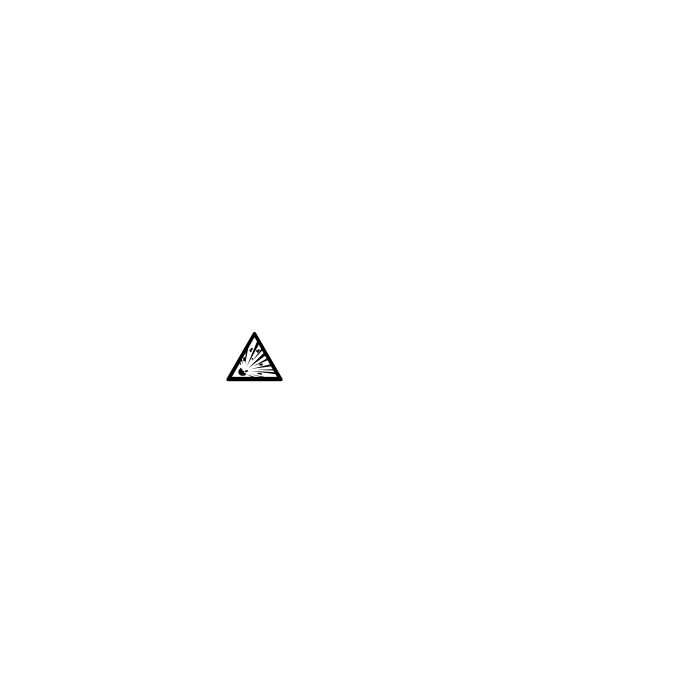
\includegraphics[height=7mm]{base/MDanger}}}\xspace}%
\newcommand{\MAttention}{\marginpar{\raisebox{-2mm}{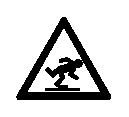
\includegraphics[height=7mm]{base/MAttention}}}\xspace}%
\newcommand{\MHint}{\marginpar{\raisebox{-2.25mm}{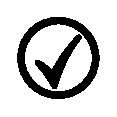
\includegraphics[height=7mm]{base/MHint}}}\xspace}%
\newcommand{\MQuestion}{\marginpar{\raisebox{-2.25mm}{
\includegraphics[height=7mm]{base/MQuestion}}}\xspace}%

% same footnote number as last one
\newcommand{\oldfootnotemark}[1]{\addtocounter{footnote}{-#1}\footnotemark\addtocounter{footnote}{#1-1}}%
%\newcommand{\lastfootnotemark}{\addtocounter{footnote}{-1}\footnotemark}%

% value-unit commands (for 457 kHz, etc)
\newcommand{\vu}[2]{\mbox{\ensuremath{#1\,\text{#2}}}}% "value-unit" ... prevents e.g. 456 \linebreak mV
\newcommand{\vuc}[3]{\mbox{\ensuremath{#1\,\text{#2}\;#3\,\%}}} % "value~unit~tolerance-per-cent"
\newcommand{\vum}[3]{\mbox{\ensuremath{#1\,\text{#2}\;#3\,\perthousand}}} % "value~unit~tolerance-per-mil"

% reminders
\newcommand{\reminder}[1]{\colorbox{red}{#1}\xspace}%
\newcommand{\rem}{\reminder{(...)}}% shortcut for the full reminder
\newcommand{\remq}{\reminder{???}}% open question
\newcommand{\remc}{\reminder{[?]}}% open citation
\newcommand{\uc}{\nxtpar\colorbox{yellow}{... under construction ...}\nxtpar}%

% misc
\newcommand{\pwd}{.} % present working directory (can be used to create relativ paths per part, etc.)




% **************************************************************************************************
% * MATH
% **************************************************************************************************

% highlighting
\newcommand{\vm}[1]{\ensuremath{\bm{#1}}}% vector or matrix

% functions
\renewcommand{\exp}[1]{\ensuremath{\text{e}^{#1}}}% exponential
\renewcommand{\ln}[1]{\ensuremath{\text{ln}\!\left(#1\right)}}% natural logarithm
\newcommand{\ld}[1]{\ensuremath{\text{ld}\!\left(#1\right)}}% logarithm base 2
\renewcommand{\log}[1]{\ensuremath{\text{log}\!\left(#1\right)}}% logarithm (base 10)
\newcommand{\logb}[2]{\ensuremath{\text{log}_{#1}\!\left(#2\right)}}% logarithm base ...

% rounding
\newcommand{\round}[1]{\ensuremath{\text{round}\!\left(#1\right)}}% rounding towards next integer
\newcommand{\ceil}[1]{\ensuremath{\left\lceil#1\right\rceil}}% rounding towards infinity
\newcommand{\floor}[1]{\ensuremath{\left\lfloor#1\right\rfloor}}% rounding towards zero

% operators
\newcommand{\E}[1]{\ensuremath{\text{E}\!\left\{#1\right\}}}% expectation operator
\newcommand{\F}[1]{\ensuremath{\mathcal{F}\!\left\{#1\right\}}}% Fourier transform operator
\newcommand{\IF}[1]{\ensuremath{\mathcal{F}^{-1}\!\left\{#1\right\}}}% inverse Fourier transform operator
\newcommand{\var}[1]{\ensuremath{\text{var}\!\left\{#1\right\}}}% variance operator
\newcommand{\cov}[1]{\ensuremath{\text{cov}\!\left\{#1\right\}}}% covariance operator
\newcommand{\corr}[1]{\ensuremath{\text{corr}\!\left\{#1\right\}}}% correlation operator
\newcommand{\avg}[1]{\ensuremath{\text{avg}\!\left\{#1\right\}}}% averaging operator
\newcommand{\avgvar}[1]{\ensuremath{\overline{\text{var}}\!\left\{#1\right\}}}% average variance operator
\renewcommand{\Re}[1]{\ensuremath{\text{Re}\!\left\{#1\right\}}}% real part
\renewcommand{\Im}[1]{\ensuremath{\text{Im}\!\left\{#1\right\}}}% imaginary part

% numbers
\newcommand{\REAL}{\ensuremath{\mathbb{R}}}% real numbers
\newcommand{\NATURAL}{\ensuremath{\mathbb{N}}}% natural numbers
\newcommand{\INTEGER}{\ensuremath{\mathbb{Z}}}% integer numbers (natural numbers plus zero)
\newcommand{\COMPLEX}{\ensuremath{\mathbb{C}}}% complex numbers
\newcommand{\IMAG}{\ensuremath{\mathbb{I}}}% imaginary numbers

% other
\newcommand{\conj}{\ensuremath{^\ast}}% conjugate complex
\newcommand{\transp}{\ensuremath{^\text{T}}}% conjugate (Hermitian) transpose
\newcommand{\mtx}[2]{\left[\ensuremath{\begin{array}{#1}#2\end{array}\right]}}%vector/matrix
\newcommand{\isdef}{\ensuremath{\mathrel{:=}}}% definition left->right
\newcommand{\isdefflip}{\ensuremath{\mathrel{=:}}}% definition right->left
\newcommand{\isreq}{\ensuremath{\mathrel{\stackrel{!}{=}}}}% is required
\newcommand{\textrel}[1]{\ensuremath{{\;{#1}\;}}}% relation symbol for in-line equations (fixed spacing)



% **************************************************************************************************
% * FLOATS (FIGURES, TABLES, LISTINGS, ...)
% **************************************************************************************************

% figures without frames
%   standard
\newcommand{\fig}[3]{\begin{figure}\centering\includegraphics[width=\textwidth]{#1}\caption{#2}\label{fig:#3}\end{figure}}%
%   with controllable parameters
\newcommand{\figc}[4]{\begin{figure}\centering\includegraphics[#1]{#2}\caption{#3}\label{fig:#4}\end{figure}}%
%   two subfigures
\newcommand{\twofig}[6]{\begin{figure}\centering%
\subfigure[#2]{\includegraphics[width=0.495\textwidth]{#1}}%
\subfigure[#4]{\includegraphics[width=0.495\textwidth]{#3}}%
\caption{#5}\label{fig:#6}\end{figure}}%
%   two subfigures with labels for each subplot
\newcommand{\twofigs}[8]{\begin{figure}\centering%
\subfigure[#2]{\includegraphics[width=0.495\textwidth]{#1}\label{fig:#8#3}}%
\subfigure[#5]{\includegraphics[width=0.495\textwidth]{#4}\label{fig:#8#6}}%
\caption{#7}\label{fig:#8}\end{figure}}%
%   two subfigures and controllable parameters
\newcommand{\twofigc}[8]{\begin{figure}\centering%
\subfigure[#3]{\includegraphics[#1]{#2}}%
\subfigure[#6]{\includegraphics[#4]{#5}}%
\caption{#7}\label{fig:#8}\end{figure}}%

% framed figures
%   standard
\newcommand{\figf}[3]{\begin{figure}\centering\fbox{\includegraphics[width=\textwidth]{#1}}\caption{#2}\label{fig:#3}\end{figure}}%
%   with controllable parameters
\newcommand{\figcf}[4]{\begin{figure}\centering\fbox{\includegraphics[#1]{#2}}\caption{#3}\label{fig:#4}\end{figure}}%
%   two subfigures
\newcommand{\twofigf}[6]{\begin{figure}\centering%
\fbox{\subfigure[#2]{\includegraphics[width=0.495\textwidth]{#1}}}%
\fbox{\subfigure[#4]{\includegraphics[width=0.495\textwidth]{#3}}}%
\caption{#5}\label{fig:#6}\end{figure}}%
%   two subfigures with labels for each subplot
\newcommand{\twofigsf}[8]{\begin{figure}\centering%
\fbox{\subfigure[#2]{\includegraphics[width=0.495\textwidth]{#1}\label{fig:#8#3}}}%
\fbox{\subfigure[#5]{\includegraphics[width=0.495\textwidth]{#4}\label{fig:#8#6}}}%
\caption{#7}\label{fig:#8}\end{figure}}%
%   two subfigures and controllable parameters
\newcommand{\twofigcf}[8]{\begin{figure}\centering%
\fbox{\subfigure[#3]{\includegraphics[#1]{#2}}}%
\fbox{\subfigure[#6]{\includegraphics[#4]{#5}}}%
\caption{#7}\label{fig:#8}\end{figure}}%

% listings
\newcommand{\filelisting}[4]{\lstinputlisting[print=true,language=#1,caption={#3},label={lst:#4}]{#2}}

% preserve backslash for linebreaks in tables (ragged... redefines \\, thus it has to be preserved)
\newcommand{\pbs}[1]{\let\temp=\\#1\let\\=\temp}%


% **************************************************************************************************
% * MISC
% **************************************************************************************************

% slighly darkened colors for text
\definecolor{bkred}{rgb}{0.9,0,0}
\definecolor{bkgreen}{rgb}{0,0.67,0}
\definecolor{bkblue}{rgb}{0,0,0.75}
% \graphicspath{{./drawings/}{./plots/}{./images/}}
% **************************************************************************************************
% ATTENTION: There is a stylesheet provided for makeindex; set makeindex to -s "./base/index.sty"
% **************************************************************************************************

% uncomment to get watermarks:
% \usepackage[first,bottom,light,draft]{draftcopy}
% \draftcopyName{ENTWURF}{160}


% **************************************************************************************************
% information fields

% general
\newcommand{\DocumentTitle}{General Information}
\newcommand{\DocumentSubtitle}{}
\newcommand{\ShortTitle}{Overview} % used in headers (keep short!)
\newcommand{\DocumentAuthor}{Fabian Moik (1430095)}
\newcommand{\DocumentDate}{Graz, \today}
%    for thesis only (will be ignored for reports)
\newcommand{\ThesisType}{Bachelor Thesis}
%\newcommand{\Organizations}{Signal Processing and Speech Communications Laboratory \\ Graz University of Technology, Austria \\[1cm] in co-operation with \\ A Nice Company \\ Cartagena, Spain} % SPSC \\ TUG \\[1cm] in cooperation with \\ A Nice Company
%\newcommand{\Supervisors}{Assoc.Prof. Dipl.-Ing. Dr. Klaus Witrisal \\ Dipl.-Ing. Paul Meissner} % Supervisor 1 \\ Supervisor 2 \\ ...
%\newcommand{\Assessors}{Univ.-Prof. Dipl.-Ing. Dr.techn. Gernot Kubin \\ Assoc.Prof. Dipl.-Ing. Dr. James J. Tobe Defined}
%\newcommand{\SpecialNote}{This work was funded by the Austrian Research Promotion Agency (FFG) under grant 123456.}
%   for report only: revision number
\newcommand{\RevPrefix}{alpha~}
\newcommand{\RevLarge}{1}
\newcommand{\RevSmall}{0}

% confidential? (can of course also be used for other messages/notes)
\newcommand{\ConfidNote}{\today}


% **************************************************************************************************
% miscellaneous

% correct bad hyphenation
\hyphenation{}
\usepackage{tabularx}
\usepackage{amsmath}
\usepackage{grffile}
\usepackage{float}
\usepackage{blindtext, graphicx}
\usepackage[labelfont=bf]{caption}
\usepackage{chngcntr}
\usepackage{mathtools}
\usepackage{hyperref}
\usepackage{pst-poker}
\psset{inline=symbol}
\psset{colorset=4c}

% switches
\newboolean{OptDraftMode}
\newboolean{DisplayContentBoxes}
% \setboolean{OptDraftMode}{true} % optional draft mode for pixel graphics (speed up generation; add \OptDraft to options)
% \setboolean{DisplayContentBoxes}{true} % optional boxes with contents (\ContentBox{Content}{NumPages} can be used as "sticky note" with planned contents)
%   load
% **************************************************************************************************
% ** SPSC Report and Thesis Template
% **************************************************************************************************
%
% ***** Authors *****
% Daniel Arnitz, Paul Meissner, Stefan Petrik
% Signal Processing and Speech Communication Laboratory (SPSC)
% Graz University of Technology (TU Graz), Austria
%
% ***** Changelog *****
% 0.1   2012-07-20   \OptDraft and \ContentBox
%
% ***** Todo *****
%
% **************************************************************************************************


% optional boxes with intended contents or other comments (can be switched on/off)
\newcommand{\ContentBox}[2]{\ifthenelse{\boolean{DisplayContentBoxes}}{\FloatBarrier\nxtpar\colorbox{yellow}{\parbox{\textwidth}{\footnotesize#1\par\hrulefill\par Number of pages: #2}}\nxtpar}{}}

% optional draft mode for large graphics (add \OptDraft to parameters for \includegraphics)
\ifthenelse{\boolean{OptDraftMode}}{\newcommand{\OptDraft}{draft}}{\newcommand{\OptDraft}{keepaspectratio}}

\renewcommand*{\thesection}{\arabic{section}}
\newcommand*{\xchapter}{\setcounter{section}{0}\addchap}
% **************************************************************************************************
% **************************************************************************************************
%
 %**************************************************************************************************
\begin{document}
%%%%%%%%% begin snippet
%% You need to add the package "tabularx".
%% Place the snippet right after \begin{document}

% need tabularx
%\usepackage{tabularx}

\begin{titlepage}
       \begin{center}
             \begin{huge}
				   %% Update assignment number here
                   \textbf{Research and General Information}
             \end{huge}
       \end{center}
       \begin{center}
             \begin{large}
                  Bachelor Thesis, 2017
             \end{large}
       \end{center}
       \begin{center}
             \begin{large}
                 \textbf{Fabian Moik}
             \end{large}
       \end{center}
\end{titlepage}

%%%%%%%%% end snippet
% **************************************************************************************************
% titlepage
%\input{./base/titlepage_\DocumentType}\emptydoublepage

% for thesis: switch to frontmatter
%\ifthenelse{\equal{\DocumentType}{thesis}}{\pagestyle{empty}\pagenumbering{roman}}{}


% **************************************************************************************************
% **************************************************************************************************
% user-defined part

% FOR THESIS: ADD THE PREAMBLE (ABSTRACT, KURZFASSUNG, ...) HERE (also add an \emptydoublepage in between), e.g.:
%    \input{my-abstract}
%    \emptydoublepage
%    \input{my-kurzfassung}
%    \emptydoublepage
%    ...
% FEEL FREE TO USE \emptypage AND \emptydoublepage TO ADJUST THE LAYOUT
% USE \thispagestyle{empty} for abstract, etc.

% for thesis: statutory declaration
\ifthenelse{\equal{\DocumentType}{thesis}}{% **************************************************************************************************
% ** SPSC Report and Thesis Template
% **************************************************************************************************
%
% ***** Authors *****
% Daniel Arnitz, Paul Meissner, Andreas Laesser, Stefan Petrik
% Signal Processing and Speech Communication Laboratory (SPSC)
% Graz University of Technology (TU Graz), Austria
%
% ***** Changelog *****
% 0.1   2010-02-18   created
% 0.2   2010-03-02   added German declaration
% 0.3   2010-06-05   removed \pagenumbering
% 0.4   2011-04-27   bugfix: \cleardoublepage replaced by \emptydoublepage
%
% ***** Todo *****
% **************************************************************************************************

\emptydoublepage \thispagestyle{empty} \vspace*{1cm}

% English
\ifthenelse{\equal{\DocumentLanguage}{en}}{
\begin{center}\Large\bfseries Statutory Declaration\end{center}\vspace*{1cm}
\noindent I declare that I have authored this thesis independently, that I have not used other than the declared sources$/$resources, and that I have explicitly marked all material which has been quoted either literally or by content from the used sources.
\par\vspace*{4cm}
\centerline{
\begin{tabular}{m{1.5cm}cm{1.5cm}m{3cm}m{1.5cm}cm{1.5cm}}
\cline{1-3} \cline{5-7}
 & date & & & & (signature) &\\
\end{tabular}}
}

% % German
% \ifthenelse{\equal{\DocumentLanguage}{de}}{
% \begin{center}\Large\bfseries Eidesstattliche Erkl�rung\end{center}\vspace*{1cm}
% Ich erkl�re an Eides statt, dass ich die vorliegende Arbeit selbstst�ndig verfasst, andere als die angegebenen Quellen$/$Hilfsmittel nicht benutzt, und die den benutzten Quellen w�rtlich und inhaltlich entnommene Stellen als solche kenntlich gemacht habe.
% \par\vspace*{4cm}
% \centerline{
% \begin{tabular}{m{1.5cm}cm{1.5cm}m{3cm}m{1.5cm}cm{1.5cm}}
% \cline{1-3} \cline{5-7}
%  & Graz, am & & & & (Unterschrift) &\\
% \end{tabular}}
% }

}{}

% TOC
%\emptydoublepage
\tableofcontents

% for thesis: make sure we switch back to standard pagestyles/numbering
\ifthenelse{\equal{\DocumentType}{thesis}}{\emptydoublepage\pagestyle{scrheadings}\pagenumbering{arabic}\mainmatter}

% FOR THESIS: YOU CAN SET THE PAGECOUNTER HERE TO MAKE IT IDENTICAL TO THE PDF PAGE NUMBER
\ifthenelse{\equal{\DocumentType}{thesis}}{\setcounter{page}{7}}{}



%%%%%%%%%%%%%%%%%%%%%%%%%%%%%%%%%%%%%%%%%%%%%%%%%%%%%%%%%%%%%%%%%

% **************************************************************************************************
% mainmatter
\newpage
% %%%%%%%%%%%%%%%%%%%%% 	1	 %%%%%%%%%%%%%%%%%%%%%%%%%
%    \emptydoublepage %FOR THESIS: ALWAYS START CHAPTERS AT RIGHT SIDE
\counterwithin{figure}{section}
\counterwithin{section}{chapter}

%%%%%%%%%%%%%%%%%% What I want to write %%%%%%%%%%%%%%%%%%%%
\chapter{State of the Art}

\section{Requirements for a Poker Playing Agent}
The main reason why creating a poker-playing system which plays at a high level is hard, is the fact that poker is a game of imperfect information \cite{nn_impl}.
A reasonably good poker bot needs to fulfill a set of requirements which includes \textbf{hand strength evaluation}, \textbf{hand potential}, \textbf{betting strategy}, \textbf{bluffing} and \textbf{opponent modeling}. Furthermore it needs to stay \textbf{unpredictable} for the opponents.\cite{key_components}\\
Some of these requirements may be handled indirectly by the poker-playing system, rather than explicitly by design. Nonetheless all of the requirements must be solved at least in some way for the system to succeed against the best human players. There are many approaches for solving each requirement and it is yet not possible to say which approach is best for which requirement. \cite{phd_poker}
\subsection{Hand Strength Estimation}
In its simplest form it is used to determine the probability of winning a hand, given the current board texture (community cards) and the hole cards of the player.
The \textbf{most successful} methods are using a \textbf{Monte Carlo Sampling} technique. The idea behind this method is to sample the remaining unknown cards and play the hand to the end. After a sufficient number of iterations the wins are counted and the hand strength is therefore estimated. In addition more factors could be taken into account such as the \textit{number of players still in the game},  \textit{hero's position at the table} and the \textit{betting action} until the current point in the game \cite{key_components}.
\subsection{Hand Potential}
Hand potential describes the probability of a hand improving or getting beat as further community cards get into play on later streets. At it's core hand potential is a function of hero's hole cards and the already dealt community cards. For an even better calculation all factors described in the hand strength estimation could be used in addition \cite{key_components}.
\subsection{Bluffing}
Bluffing is essential to succeed in the game of poker. From a game theoretical point of view, there is an optimal bluffing frequency in certain situations. A system with a minimal bluffing strategy would bluff exactly that percentage of hands randomly. However, a better bluffing strategy would identify profitable bluffing opportunities by predicting the probability of an opponent to fold. \cite{phd_poker}
\subsection{Unpredictability}
This part of the system allows to hide information from the opponents by varying strategies for a given situation over time. \cite{phd_poker}
\subsection{Opponent Modeling}
Opponent modeling describes the method of modeling a likely probability distribution of the opponent's hand. In it's simplest form a single generic model could be used for all opponents. However, to improve the system the probabilities can be modified based on the collected data of each opponent. \cite{phd_poker}\\\\
All of these requirements combined form a \textbf{betting strategy}, which determines the optimal play whether to \textit{fold}, \textit{call} or \textit{raise} in a certain situation.
%%%%%%%%%%%%%%%%%% State-of-the-art Poker Bots %%%%%%%%%%%%%%%%%%%%
\section{Different types of poker bots}
The Annual Computer Poker Competition takes place each summer at the \textit{AAAI Conference on Artificial Intelligence} or at the \textit{International Joint Conference on Artificial Intelligence} and attracts competitors from all around the world to compete in the challenge to improve existing methods or develop new ideas and algorithms for beating complex variants of poker. \cite{acpc} \\\\
Following link redirects to the AAAI official website where results of recent competitions can be found.\\
\url{http://www.computerpokercompetition.org/}\\\\
The official University of Alberta Research Team website offers a vast majority of poker AI research and is the starting point for most novices in poker AI. Many years of research have produced a number of precious articles and papers which can be found on their website.\\
\url{http://poker.cs.ualberta.ca/index.html}\\\\

\subsection{Knowledge-based poker agents}
Knowledge-based systems can be broken into two categories, namely \textit{rule-based expert systems} and \textit{formula-based methods}. In general knowledge-based systems require the knowledge of an expert player to design the system\cite{review}.A \textbf{rule-based expert system} in its simplest form is a sequence of \textit{if-else} statements for frequently occurring scenarios of the game. Human players describe their poker hands in a very similar way when they break them down in a discussion \cite{master_nuno}. \textbf{Formula-based methods} on the other hand are a more generalized system which takes a collection of weighted inputs that describe the current game state and then outputs a probability triple upon which a betting decision is made. An example for a typical input to the formula is the hand strength and pot odds. 
\subsection{Monte-Carlo Simulation}
In general simulation based methods rely on repeatedly simulating an outcome in order to obtain a statistical average \cite{master_nuno}. A frequently used simulation method applied to the game of poker is the so called \textit{Monte-Carlo simulation or Monte-Carlo Tree Search}, which is a procedure that searches the game tree by drawing random samples for choices in a game state and simulates the play until a leaf node (last betting round when five community cards are present) is reached \cite{review}. At this point the payoff value for one path is known and the procedure is repeated until the values for intermediate nodes in the tree converge to a robust evaluation value \cite{review}.
In poker this approach can be highly volatile because the outcome of the simulation highly depend on the quality of the simulated play. Future actions in a hand are not only determined by the knowledge of the opponent's hole cards and the community cards but also on the type of opponent one is facing, hence biased values for certain situations might lead to inaccurate simulation outcomes. \cite{master_nuno}
\subsection{e-Nash Equilibrium based poker agents}
The currently best performing poker-playing programs are approximating a \textit{Nash equilibrium} \cite{nash}. In game theory, the Nash equilibrium is a solution concept of a non-cooperative game involving two or more players in which each player is assumed to know the equilibrium strategies of the other players, and no player has anything to gain by changing only his own strategy \cite{game_theory}.\\\\
The most successful bots for Heads-up No-Limit (HUNL) Hold'em poker all use the same basic structure. They are based on using a smaller abstract version of the game in which they then approximate the nash equilibrium and execute the result in the original game via a translation method. In the abstract version of the game the bot abstracts the card information by clustering hands with similar strength and potential. Furthermore it abstracts the betting information by restricting the available bets to a small number of crafted bets, dependent on the current size of the pot. \cite{nash} \\\\
The currently most used and most successful algorithm for approximating the Nash equilibrium in the abstract game is called \textbf{Counterfactual Regret Minimization}. All three top performing players in ACPC 2016 used this algorithm and outperformed the rest of the competition. \cite{nash} \\
\subsection{Exploitive poker agents}
Eventhough Nash-equilibrium approaches are static and robust strategies, they will never identify and exploit opponents' weaknesses because equilibrium strategies limit their own exploitability by assuming that they play against a perfect opponent who also plays an equilibrium style.\cite{review} To maximize the winnings against a weak opponent good poker agents attempt to adapt to their opponents' playing style by constructing accurate opponent models which alters their equilibrium play, therefore making them exploitable too.
attempt to adapt to their opponents' playing style by constructing accurate opponent models
\subsection{Bayesian poker agents and evolutionary algorithms}
\textbf{Bayesian poker agents}\\\\
A Bayesian network is a probabilistic graphical model. Each node in the directed acyclic graph represents a random variable and edges between nodes represent the conditional dependencies of variables. Nodes are associated with a probability function which returns the conditional probability values based on the values of the parent node. Initializing nodes within the network with different values results in propagated probabilities throughout the network which yield a probability distribution over the random variables. Compared to other poker playing agents, bayesian agents performed badly in the AAAI Computer Poker Competitions in the last years. There is still a lot of room for improvement in Bayesian based networks and further research in this field has to be done to stand a chance in upcoming competitions. \cite{review}\\\\
\textbf{Evolutionary Algorithms}\\\\
Evolutionary algorithms evolve a population of agents over successive generations. A \textit{fitness function} typically decides which agents are more likely to proceed to the next generation.The  offspring is then created via a \textit{crossover} procedure. Additionally a procedure called \textit{coevolution} can be used  to restrict the evolution process of a population. For this purpose separate genetic populations are maintained and evolution can only occur within these separated populations. In combination with evolutionary algorithms, neural networks are often used for the poker playing agents which compete against each other over a number of generations. The best ranking agents are then selected to act as parents for the next generation. In the crossover procedure the weights of the evolved neural networks are calculated using a biased sum over the parents' weights.\cite{review}

%%%%%%%%%%%%%%%%%%%%%%%%%%%%%%%%%%%%%%%%%%%%%%%%
\chapter{Evolutionary Neural Network}
Unlike other games such as Chess, Checkers or Go, Poker is a game of imperfect information. This means, that a player can not see all relevant  information at a given game state at all times. The game of Poker involves hidden information and deception. and therefore players must be willing to take risks, based on the information they have \cite{nn_evolve}. Imperfect information includes a very large decision space and therefore efficient computational calculations which search for the optimal decision path may be unfeasible for many problems, including the No-Limit Hold'em version of poker. Unlike other methods, which reduce the decision space by transforming the game into a smaller abstract version in which they then approximate the optimal path and  execute the result in the original game via a translation method, my approach is to use an evolutionary algorithm on agents improving their game by training a neural network through iterative play. \cite{nn_evolve}
\section{Evolutionary algorithms}
\textit{"Evolutionary algorithms mimic natural evolution, and reward good decisions while punishing less desirable ones.\cite{nn_evolve}"}
Agents make betting decisions based on given input features to the neural network, which represent the current game state as detailed as possible. The evolutionary algorithm is then applied to the neural network itself. It may add or remove certain features and change the weights of the parameters \cite{nn_evolve}. Adding random noise to the weights provides a crucial feature of natural evolution - Mutation. A small percentage of random mutation allows agents not to get stuck in local optima. Before the evolution of a population can occur the population first needs to be evaluated. To find a number of suitable parents to form the next generation all agents of the current population compete against each other in a number of tournaments where their finishing place is directly correlated to their fitness. The fittest agents are then chosen for reproduction. Together with the best agents of the previous generation the newly born agents for the new generation and once again compete against each other in a number of tournaments. The exact procedure of evolving a population has not yet been established since it \textbf{will not} be the aim of this work. The goal is rather to set up a test environment where agents can be evaluated and sorted by their strength of play.

%%%%%%%%%%%%%%%%%%%%%%%%%%%%%%%%%%%%%%%%%%%%%%%%
\chapter{Testbed}
In order to test a population of agents against each other, a suited test bed is needed. Creating a Poker playing agent requires a lot of computation and simulation. It starts with calculating the chances of winning a hand given the current state of the game considering the positive and negative hand potential for all possible opponent's hand combinations. Certain probabilities can be precalculated and saved as lookup tables others require real time calculations and simulations. Some open source libraries can be found, which help with the hand evaluation process and also offer some other handy features for creating a dynamic test bed. Such libraries and APIs are, for example,  linked on the \textit{University of Alberta Computer Poker Research Group} website. There already exist some test beds for poker playing agents but most of them do not provide simulations for tournaments or are too slow and their architecture make it hard to create or implement new agents \cite{agent_sim}. Unfortunately most of the libraries are Java libraries but since they are open source it should not be too hard to port them to other languages such as C++. On reason for building the test bed in C++ is the speed of the language and my programming  knowledge in it, compared to Java. But I have not yet decided if I want to fully implement my test bed in C++ (or Python) or try to use the existing libraries to some extend in their native language and combine both languages.\\\\
With the evolutionary approach of creating a Poker playing agent, an efficient test bed which can simulate hundreds of thousands of games per hour is needed. The general idea is to write a program which simulates a Poker tournament with \textit{x tables} and \textit{9 agents} per table. Each agent uses a neural network for its betting decisions. The inputs for the neural network are provided by a class which holds all the table information. The test bed then runs thousands of tournaments and keeps track of the final placements of each agent. After x number of tournaments, the fittest agents are selected to form a new generation. Some other features can be implemented in the simulation environment for instance a table seat permutation would reduce the variance of the end results and could hence speed-up the simulations by reducing the number of needed simulations \cite{agent_sim}. A precise explanation on the workflow of the evolutionary algorithm can not be given at this moment, because the idea of this bachelor thesis is to setup the test bed and the neural networks of the playing agents including the intense calculations of the input features to the neural network. The final goal is to use this thesis as a cornerstone for the future work on a fully functional and autonomous poker playing agent.
%%%%%%%%%%%%%%%%%%%%%%%%%%%%%%%%%%%%%%%%%%%%%%%%
\chapter{Structure and Input of Neural Network}
\section{General Structure}
At this point it is not yet decided if two neural networks will be used, one for the pre-flop game and one for the post-flop game, or if one neural network for both game stages would be sufficient. Under the assumption of two separate networks for each stage of the game the preliminary structure of the post-flop neural network consists of an input layer with 22 neurons,  one hidden layer with a yet unknown number of neurons and an output layer with three neurons. Following inputs are necessary to keep track of the evolution of the table and are listed in ~\ref{feature_tab}. The three output neurons represent the so called \textbf{probability triple} (f, c, r), which specifies the probability distribution for the actions \textit{fold, check/call} or \textit{bet/raise} at the current state of the game \cite{review}. According to this distribution an action is then chosen by the agent.

\section{Feature-List}
\begin{table}[]
\begin{tabular}{|l||l|}
\hline
\multicolumn{1}{|c||}{Input} & \multicolumn{1}{c|}{Feature} \\ \hhline{=#=}
1                           & Effective Hand Strength      \\ \hline
2                           & Chip count                   \\ \hline
3                           & Chips in pot                 \\ \hline
4                           & Chips to call                \\ \hline
5                           & Number of opponents          \\ \hline
6                           & Position of hero             \\ \hline
7-14                        & Chip count of all opponents  \\ \hline
15-22                       & Opponent model               \\ \hline
\end{tabular}
\centering
\caption{Table of inputs (features) for the neural network}
\label{feature_tab}
\end{table}
\section{Effective Hand Strength (EHS)}
The EHS in conjunction with other components should be used to help selecting a suitable betting action. It is an indicator for how likely a hand is winning at showdown considering the current hand strength but also the positive and negative hand potential.
\section{Chip count}
The second feature is the number of chips the acting agent has. 
\section{Chips in pot}
The third feature is the number of chips already in the pot, including all chips of previous betting rounds plus the number of chips betted by other agents in the current betting round. An agent may not be able to win all the chips in the pot if his chip count (stack) is smaller than a bet of his opponents in the current round. Hence the value of this feature is the effective pot size an agent can actually win when his hand is the strongest at showdown.
\section{Chips to call}
The fourth feature is the number of chips an agent has to match if it wants to continue in the hand. Combined with the third feature this forms the so called \textbf{pot odds}, which represent the bet to pot ratio and is a commonly used term and tool in the Poker community to calculate the needed winning percentage of an agent's hand to make the call a profitable play.
\section{Number of opponents}
This feature is the number of opponents currently involved in the hand.
\section{Chip counts of all players}
In a 9-handed multi table tournament there are at most 9 players on a table. Therefore this feature has 9 inputs, one for each player on the table. The input is the number of chips an opponent has. Late in a tournament it will occur that hands are not always played 9-handed but with less then 9 players per hand. For this case the input of empty seats on the table is set to unknown and will be recognized by the neural network as an empty seat.
\section{Position of hero}
This feature is the relative position of the agent to the dealer. The dealer position is the most valuable position in Poker because the action of only two more players will follow in an unopened pot. In general it is desirable to be in a late position because many players have already acted before you have to do and hence more information is available for the agent in late position.
\section{Opponent model}
The opponent model should indicate which type of opponent the agent is facing. For this purpose a combination of \textit{VPIP (Voluntarily Put Money In Pot), PFR (Pre-flop Raise)} and \textit{AF (aggression factor)} is used. The VPIP of the player is the percentage of hands in which a player voluntarily puts money in the pot, PFR is the percentage of hands in which a player puts in a pre-flop raise and the AF is the number of times a player bets plus the number of times he raises divided by the number of times he calls (Bets + Raises)/Calls. All three values together give a good estimation of the overall playing style of the opponent. In general there are four basic Poker playing styles: Tight Passive, Loose Passive, Tight Aggressive (TAG) and Loose Aggressive (LAG). Aggression is key in winning at Poker. Passive playing styles will never win at the game of poker.

%%%%%%%%%%%%%%%%%%%%%%%%%%%%%%%%%%%%%%%%%%%%%%%%
\chapter{Calculating the EHS}
To calculate the winning chances of a poker hand and comparing it with the cost of playing the hand is essential to make profitable long term decisions.
A hand evaluation algorithm tries to approximate the chances of winning a hand at a given state in the current game and a given the opponent models. Simply calculating the current hand strength is insufficient if there are community cards still to come. Therefore a good hand evaluation algorithm for post-flop play takes
the present hand strength and the hand potential on later betting streets into account.\cite{ehs}\\\\
For the pre-flop evaluation the hand potential is not considered due to the computational complexity and hence a different evaluation is used for pre-flop play.\cite{ehs}\\
At this point of time it is not yet clear which methods will be used for calculating the EHS. Since there are some open source projects which already have a hand evaluator implemented, not all calculations will be done manually. Some fast evaluators are from the GPL pokersource project and can be found on SourceForge.net. They offer hand evaluators for C, Java and Python. Though I am not yet sure how good and how well suited those 'ready to go' hand evaluators are. This is the reason why I can not yet tell how the hand evaluation will be done in this work.

\section{Pre-flop}
A hand evaluation for the pre-flop stage of the game is not very complex since there is a very limited number of possible holdings and there is little information before the flop that could influence a betting decision.Factors which play a role in the hand evaluation before the flop are the two hole cards of the player, previous player actions, opponent models from previous hands (not always given) and the position at the table relative to the dealer \cite{phd_poker}. There are a total of ${52 \choose 2})= 1326$ different hands in poker, of which many of them are equivalent before the flop \cite{opp_mod_adv}. For example a hand such as \As\twos and \Ac\twoc have the same chance of making a flush and the same overall chance of winning. With this additional information there are 169 distinct hand types left (13 paired hands, ${13 \choose 2}$ = 78 suited hands and $13 \cdot {4 \choose 2} = 78 unsuited hands$) \cite{ehs}. With a method known as \textit{roll-out simulation} tables can be calculated offline \cite{opp_mod_adv}. \\
For each of the 169 distinct hand types a simple roll-out simulation of around 1 million hands can be done against each of one to nine opponents. The opponents simply call the big blind and then check all the way to the showdown. This methods yields a statistical measure of the approximate hand strength of each starting hand. Although this method assumes a simplified scenario where each player calls to the end, it however gives a good first approximation of how strong a starting hand is. \cite{ehs}
As described in \cite{phd_poker} the simple \textit{roll-out simulation} can be refined by letting the previous results  govern the betting decision of each player. A net negative value of the income rate (IR) in the previous iteration would therefore mean, that the player should rather fold the hand instead of calling the big blind. This method would produce a more realistic distribution of opponents and would define a set of hands that can be played profitably against the blind and other unknown hands but it does nether take the betting position nor the know opponent actions into account.\cite{phd_poker} Therefore a simple \textit{roll-out simulation} could as well be sufficient for an adequate pre-flop play.


%%%%%%%%%%%%%%%%%%%%%%%%%%%%%%%%%%%%%%%%%%%%%%%%
\chapter{Basic Structure of Bachelor Thesis}
\begin{enumerate}
\item[1.)] Introduction to the Game of Poker
\begin{enumerate}
\item[1.1)] No-Limit Hold'em
\end{enumerate}
\item[2.)] Poker as a Test Bed for AI
\begin{enumerate}
\item[2.1)] History of Poker Bots
\item[2.2)] Breakdown of Obstacles in the Creation of a Poker Bot
\end{enumerate}
\item[3.)] Evolutionary Algorithms in Conjunction with Neural Networks
\begin{enumerate}
\item[3.1)] What is an Evolutionary Algorithm
\item[3.2)]  What are Neural Networks
\end{enumerate}
\item[4.)] Creating a Poker Bot Using AE and NN
\begin{enumerate}
\item[4.1)] Implementation of the Test Bed
\begin{enumerate}
\item[4.1.1)] Calculation of EHS
\end{enumerate}
\item[4.2)] Implementation of the NN Agents
\begin{enumerate}
\item[4.2.1)] Feature Set
\end{enumerate}
\item[4.3)] Testing Agents by Self-Play
\end{enumerate}
\item[5.)] Future work (Master Thesis)
\begin{enumerate}
\item[5.1)] Using EA to Make a Strong Poker Playing Agent
\end{enumerate}
\end{enumerate}

% **************************************************************************************************
%\appendix
%\bibliographystyle{./base/IEEEtran}
%\bibliography{_bibliography}
\begin{thebibliography}{9}
\bibitem{key_components}
  Darse Billings et al.,
  \textit{Using Selective-Sampling Simulations in Poker},
  Department of Computing Science - University of Alberta, Edmonton,
  Alberta Canada,
  1999.
\bibitem{phd_poker}
  Darse Billings et al.,
  \textit{The Challenge of Poker},
  Department of Computing Science - University of Alberta, Edmonton,
  Alberta Canada,
  June 22, 2001.
\bibitem{dis_poker}
  Darse Billings ,
  \textit{Algorithms and assessment in computer poker},
  Department of Computing Science - University of Alberta, Edmonton,
  Alberta Canada,
  2006.
\bibitem{nash}
  Viliam Lisy and Michael Bowling ,
  \textit{Eqilibrium Approximation Quality of Current No-Limit Poker Bots},
  Department of Computing Science - University of Alberta, Alberta Machine Intelligence Institute,
  Jan. 8, 2017.
\bibitem{acpc}
  Super User( Dec. 27, 2012).
  \textit{About the ACPC}. Retrieved from http://www.computerpokercompetition.org/index.php/about,
\bibitem{nn_impl}
  Tjebbe Laurens Vlieg,
  \textit{Computer Poker with Neural Networks},
  University of Amsterdam - Faculty of Science, 
  June 26, 2012.
\bibitem{master_nuno}
  Nuno Miguel da Silva Passos,
  \textit{Poker Learner: Reinforcement Learning Applied to Texas Hold'em Poker},
  Faculdade de Engenharia da Universidade do Porto, 
  July 18, 2011.
\bibitem{nn_evolve}
  Garrett Nicolai and Robert Hilderman,
  \textit{Algorithms for Evolving No-Limit Texas Hold'em Poker Playing Agents},
  Dalhousie University, Halifax, Canada; Department of Computer Science, University of Regina, Regina, Canada, 
  Sep, 2010.
\bibitem{ehs}
  Danis Richard Papp,
  \textit{Dealing with Imperfect Information in Poker},
  University of Alberta, 
 Fall, 1998.
\bibitem{opp_mod}
  Darse Billings, Denis Papp, Jonathan Schaeffer, Duane Szafron,
  \textit{Opponent Modeling in Poker},
  Department of Computing Science, University of Alberta, 
 1998.
\bibitem{review}
 Jonathan Rubin, Ian Watson,
  \textit{Computer poker: A review},
  Department of Computing Science, University of Auckland, New Zealand, 
 Jan. 21, 2011.
\bibitem{opp_mod_adv}
Aaron Davidson, 
  \textit{Opponent Modeling in Poker: Learning and Acting in a Hostile and Uncertain Environment},
  Department of Computing Science, University of Alberta, 
 Summer, 2002.
\bibitem{agent_sim}
Francesca Giardini, Frederic Amblard, 
  \textit{Multi-Agent-Based Simulation XIII},
 Springer, Revised Selected Papers, International Workshop MABS, 
 June, 2012.
\bibitem{game_theory}
Martin J. Osborne, Ariel Rubinstein, 
  \textit{A Course in Game Theory},
 The MIT Press, Cambridge, Massachusetts, London, England, 
 Jan. 07, 2014.
\end{thebibliography}
% **************************************************************************************************
% **************************************************************************************************

% place all floats and create label on last page
\FloatBarrier\label{end-of-document}
\end{document}

